\subsection{Ćwiczenie dydaktyczne --- Kodowanie Reeda-Solomona}

\subsubsection{Wstęp teoretyczny}
Kodowanie korekcyjne Reeda-Solomona zostało stworzone przez Irvina S. Reeda
oraz Gustava Solomona w 1960 roku.
Kody Reeda-Solomona charakteryzują się kilkoma parametrami:
\begin{itemize}
    \item alfabetem w ciele skończonym $\mathbb{F}_{2^m}$, $m>1$
    \item długością wiadomości $k$ do zakodowania $k < 2^{m}$
    \item długością słowa kodowego $n$ gdzie $k < n < 2^{m}$
    \item wielomianem generującym $g(x)$
\end{itemize}

Kody Reeda-Solomona cechują się możliwością korekty $\lfloor \frac{n-k}{2} \rfloor$
lub wykrycia $n-k$ błędnych symboli. Symbol w ciele $\mathbb{F}_{2^m}$ składa się
z $m$ bitów co w przypadku błędów grupowych daje możliwość korekty maksymalnie
$m \cdot \lfloor \frac{n-k}{2} \rfloor$ bitów bądź detekcji $m(n-k)$ przekłamanych bitów

Aby zrozumieć działanie kodu Reeda-Solomona trzeba najpierw zrozumieć
czym jest ciało skończone $\mathbb{F}_q$ zwane też ciałem Galois $\operatorname{GF}(q)$.

\paragraph{Ciało skończone $\mathbb{F}_q$}

Ciało to jest ciałem $K$ rzędu $q$ czyli takie które zawiera jedynie $q$ elementów. Aby ciało skończone istniało $q$ musi spełniać warunek $q=p^k$, $k \in \{ 1, 2, \ldots \}$ gdzie $p$ jest liczbą pierwszą oraz definiować działania dodawania i mnożenia spełniające kilka warunków:
\begin{itemize}
    \item dodawanie i mnożenie jest łączne, przemienne oraz zawiera elementy neutralne
    \item każdy element musi posiadać element odwrotny względem dodawania
    \item każdy element oprócz $0$ musi posiadać element odwrotny względem mnożenia
    \item mnożenie jest rozdzielne względem dodawania
\end{itemize}

Aby stworzyć ciało $\mathbb{F}_p$ gdzie $p$ jest liczbą pierwszą można wykorzystać pierścień klas reszt $\modulo{p}$ w którym działania to zwykłe dodawanie i mnożenie modulo
\begin{align*}
    \modulo{p} = \{ [a]_p \; | \; a \in \mathbb{Z} \} &= \{ [0]_p, [1]_p,
    [2]_p, \ldots, [p-1]_p \} \\
    [a]_p + [b]_p &= [a + b]_p \\
    [a]_p \cdot [b]_p &= [a \cdot b]_p
\end{align*}

W tym wprowadzeniu będą używane jedynie ciała $\mathbb{F}_2$ oraz $\mathbb{F}_{2^m}$ z których korzysta kod Reeda-Solomona.

\paragraph{Ciało $\mathbb{F}_2$}

Ciało $\mathbb{F}_2$ jest jednym z najczęściej używanych ciał w informatyce. Ciało to definiuje 2 elementy $\{ 0, 1 \}$ w którym działania $+$ i $\cdot$ są równoważne operacjom logicznym XOR oraz AND
\begin{table}[H]
    \captionof*{table}{Dodawanie i mnożenie w $\mathbb{F}_2$}
    \centering
    \begin{tabular}{c c | c c}
        \toprule
        a & b & $+$ & $\cdot$ \\
        \midrule
        0 & 0 & 0 & 0 \\
        \midrule
        0 & 1 & 1 & 0 \\
        \midrule
        1 & 0 & 1 & 0 \\
        \midrule
        1 & 1 & 0 & 1 \\
        \bottomrule
    \end{tabular}
\end{table}


\paragraph{Ciało $\mathbb{F}_{2^m}$}

Aby zdefiniować ciało skończone $\mathbb{F}_{2^m}$ potrzebujemy najpierw
znaleźć wielomian nierozkładalny $p(x)$ stopnia $m$, czyli taki który nie
da się przedstawić jako iloczyn dwóch innych wielomianów stopnia
mniejszego $p(x) = g(x) \cdot f(x)$

Wielomian jest ten potrzebny do zdefiniowania działania mnożenia ponieważ elementy tego ciała interpretowane są jako wielomiany w postaci:
\begin{align*}
    \sum_{n=0}^{m-1} c_n \alpha^n = c_{0} + c_{1}\alpha + c_{2}\alpha^{2} + \cdots + c_{m-1}\alpha^{m-1},
    c_{n} \in \mathbb{F}_2
\end{align*}

Wielomiany te mogą być reprezentowane jako liczby binarne $c_{m-1} c_{m-2} \ldots c_{1} c_{0}$ bądź po konwersji liczby binarnej jako np.\ liczby dziesiętne. Przykładowe wielomiany w ciele $\mathbb{F}_{2^4}$ i ich różne zapisy podane są w tabelce:
\begin{table}[hp]
    \captionof*{table}{Interpretacje niektórych elementów ciała $\mathbb{F}_{2^4}$}
    \centering
    \begin{tabular}{c c c}
        \toprule
        Wielomian & Liczba Binarna & Liczba dziesiętna \\
        \midrule
        $x^3 + x^2 + x + 1$ & 1111 & 15 \\
        \midrule
        $x^3 + x$ & 1010 & 9 \\
        \midrule
        $x + 1$ & 11 & 3 \\
        \bottomrule
    \end{tabular}
\end{table}

Dodawanie elementów w ciele $\mathbb{F}_{2^m}$ jest po prostu zwykłym dodawaniem wielomianów, trzeba tylko pamiętać, że współczynniki dodajemy w ciele $\mathbb{F}_2$ czyli XORujemy:
\begin{align*}
    \sum_{n=0}^{m-1} c_n \alpha^n + \sum_{n=0}^{m-1} d_n \alpha^n =
    \sum_{n=0}^{m-1} (c_n + d_n) \alpha^n
\end{align*}
Wynikiem mnożenia $a$ i $b$ w ciele $\mathbb{F}_{2^m}$ jest reszta z
dzielenia iloczynu tych wielomianów przez wielomian nierozkładalny $p(x)$.
Dzielenie jak i mnożenie można wykonać tak jak na zwykłych wielomianach, pamiętając o tym, że współczynniki są w ciele $\mathbb{F}_2$.
\newline
Przykładowe działanie mnożenia w $\mathbb{F}_{2^2}$, wielomian nierozkładalny $p(x)=x^2 + x + 1$

\begin{align*}
    a &= \alpha + 1 \text{, } b = \alpha + 1 \\
    a \cdot b &= (\alpha + 1)^2 &\mod x^2 + x + 1 \\
    a \cdot b &= \alpha^2 + [2]_{2}x + 1 &\mod x^2 + x + 1 \\
    a \cdot b &= \alpha^2 + 1 &\mod x^2 + x + 1 \\
    a \cdot b &= \alpha
\end{align*}

Zamiast liczenia reszty z dzielenia można także skorzystać z pewnej zależności. Zdefiniujmy $\alpha$ jako pierwiastek wielomianu $p(x)$.
\begin{align*}
    [-1]_2 &\equiv [1]_2 \\
    p(\alpha) &= 0 \\
    \alpha^2 + \alpha + 1 &= 0 \\
    \alpha^2 &= -\alpha - 1 \\
    \alpha^2 &= \alpha + 1
\end{align*}

Teraz zamiast liczyć resztę z dzielenia możemy po prostu podstawić $\alpha^2$:
\begin{align*}
    a \cdot b &= \alpha^2 + 1 \\
    a \cdot b &= (\alpha + 1) + 1 \\
    a \cdot b &= \alpha
\end{align*}

\paragraph{Oryginalny kod Reeda-Solomona}
Sposób kodowania przedstawiony w pracy Reeda i Solomona polega na stworzeniu wielomianu $p_m(x)=\sum_{i=0}^{k-1}m_{i}x^i$, gdzie $m_i\in\mathbb{F}_{2^m}$
to $i$\nobreakdash-ty element wiadomości, po czym za pomocą tego wielomianu
obliczane jest słowo kodowe $C(m)=(p_m(a_0), p_m(a_1), \ldots, p_m(a_{n-1}))$
gdzie $a_i$ to różne elementy ciała $\mathbb{F}_{2^m}$.
\newline
Przykładowy kod RS dla $\mathbb{F}_{2^2}$, $p(x) = x^2 + x + 1$, $n=3$,
$k=2$, wiadomość to 2 liczby 2 i 3.

\begin{align*}
    p_m(x) &= 3x + 2 \\
    p_m(0) &= 3 \cdot 0 + 2 = 2 \\
    p_m(1) &= 3 \cdot 1 + 2 = 3 + 2 = 0\text{b}11 + 0\text{b}10 = 0\text{b}01 = 1 \\
    p_m(2) &= 3 \cdot 2 + 2 = (\alpha + 1) \cdot \alpha + \alpha \\
    p_m(2) &= 3 \cdot 2 + 2 = \alpha^2 + \alpha + \alpha = \alpha + 1 = 3 \\
    p_m(3) &= 3 \cdot 3 + 2 = (\alpha + 1)^2 + \alpha = \alpha + \alpha = 0
\end{align*}

Zakodowana wiadomość to ``2 1 3 0''

\paragraph{Kod systematyczny}

Za pomocą niewielkiej modyfikacji można stworzyć kod systematyczny czyli taki w którym słowo kodowe zawiera w sobie kodowaną wiadomość.
Żeby stworzyć kod systematyczny musimy zmodyfikować sposób tworzenia wielomianu w taki sposób by $p_m(x_i)=m_i$ dla $i \in \{0,1,\ldots,k-1\}$.

Jednym ze sposobów stworzenia takiego wielomianu jest użycie metody interpolacji wielomianów. Słowo kodowe wygenerowane z tego wielomianu będzie zawierało wiadomość w pierwszych $k$ elementach.
\[C(m)=(p_m(a_0), p_m(a_1), \ldots, p_m(a_{n-1}))=(m_0, m_1, \ldots, m_{k-1}, p_m(a_k), p_m(a_{k+1}), \ldots, p_m(a_{n-1}))\]

\paragraph{kod BCH}

Kody BCH~(Bose-Chaudhuri-Hocquenghem) są kodami cyklicznymi co oznacza że każde przesunięcie słowa kodowego jest także słowem kodowym np.
\begin{align*}
    (c_0, c_1,\ldots, c_{n-2}, c_{n-1})\text{, }(c_{n-1}, c_0, \ldots, c_{n-3}, c_{n-2})
\end{align*}

Aby zbudować kod BCH Reeda-Solomona potrzebujemy najpierw funkcji minimalnej pierwiastka $\alpha$, czyli takiego minimalnego wielomianu nierozkładalnego $p(x)$ stopnia $m$ dla którego istnieje element prymitywny~(pierwiastek) $\alpha$ który pozwala wygenerować całe ciało skończone
\begin{align*}
    \mathbb{F}_{2^m} = \{0, 1, \alpha, \alpha^2, \ldots, \alpha^{p^{m}-1} \}
\end{align*}

Mając taki element prymitywny jesteśmy w stanie stworzyć wielomian generujący $g(x)$ używając wzoru
\begin{align*}
    t &= n - k \\
    g(x) = \prod_{i=0}^{t-1} (x - \alpha^i) &= g_{t}x^t + g_{t-1}x^{t-1} +
    \cdots + g_{1}x + g_{0}
\end{align*}
Aby utworzyć słowo kodowe wystarczy pomnożyć wielomian $p_m(x)$ przez wielomian generujący $g(x)$

\paragraph{systematyczny kod BCH}\label{systematic-bch-rs}

Aby uzyskać systematyczne słowo kodowe $s(x)$ musimy obliczyć:
\begin{align*}
    s_r(x) &= p_m(x) \cdot x^t \mod g(x) \\
    s(x) &= p_m(x) \cdot x^t - s_r(x)
\end{align*}

\subsubsection{Narzędzia}
\paragraph{Reed-Solomon}
\begin{center}
    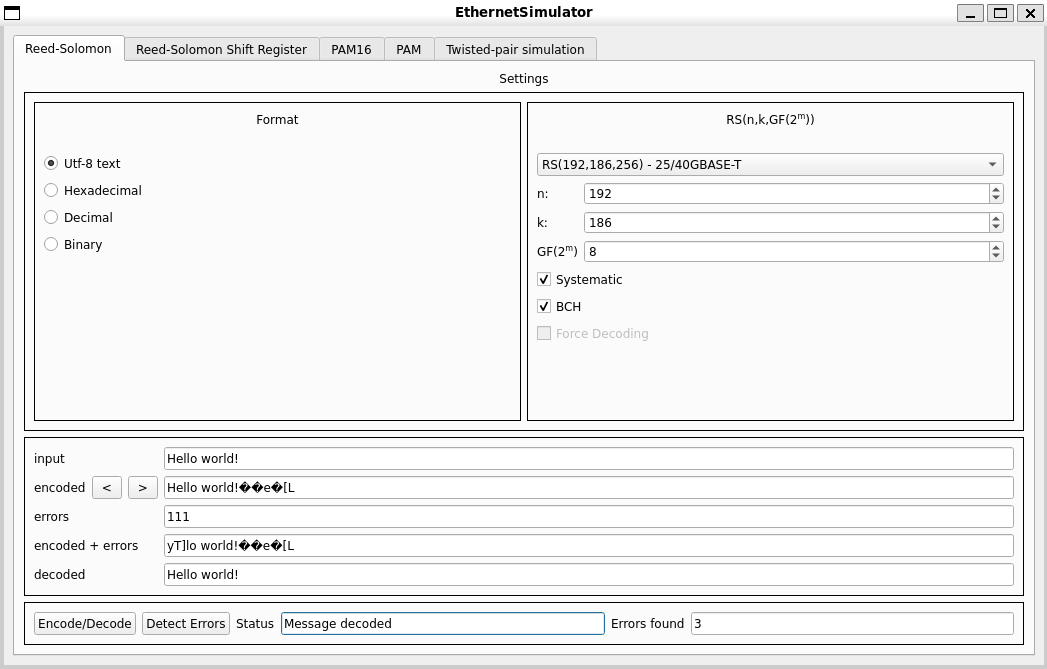
\includegraphics[width=0.95\textwidth,keepaspectratio]{rs-tab.png}
\end{center}
Narzędzie pozwala na:
\begin{itemize}
    \item Kodowanie i dekodowanie wiadomości różnymi koderami o różnych
    parametrach
    \item Nakładanie na zakodowaną wiadomość błędów w celu przetestowania
    możliwości detekcji i korekty błędów przez kod Reeda-Solomona
    \item Zmianę formatu symboli w celu łatwiejszego zobrazowania co się
    dzieje w poszczególnych etapach
\end{itemize}

Zakładka Reed-Solomon składa się z 3 części
\begin{itemize}
    \item Format --- pozwala na zmianę formatu wyświetlanych danych.
    Tryb tekstowy pozwala na szybkie zorientowanie się jak dane się
    zmieniają. Tryb binarny pozwoli na dokładne dodanie błędów do
    słowa kodowego. Kodowanie znaków tekstowych to UTF-8 w związku z
    czym polskie znaki diakrytyczne kodowane są na 2 bajtach.
    \item RS($n$, $k$, $GF(2^m)$) --- parametry kodu
    RS~(wielomian $p(x)$ jest obliczany automatycznie).
    \item Dane --- tutaj możemy wpisać wiadomość którą chcemy
    zakodować lub błędy które będą XORowane ze słowem kodowym oraz
    zobaczyć wynik kodowania. Status informuje nas o tym czy
    znaleziono błędy bądź czy udało się zdekodować wiadomość.
    `Errors found' informuje ile błędów zostało poprawionych.
\end{itemize}

Tryb tekstowy nie jest w stanie poprawnie wyświetlić wszystkich
znaków, część jest zamieniana na znaki zapytania a część jest tzw.
~znakami białymi (spacje, tabulatory bądź znaki niewyświetlane).
Strzałki przy `encoded' pozwalają na przesunięcie symboli w lewo i prawo.

\paragraph{Reed-Solomon Shift Register}
\begin{center}
    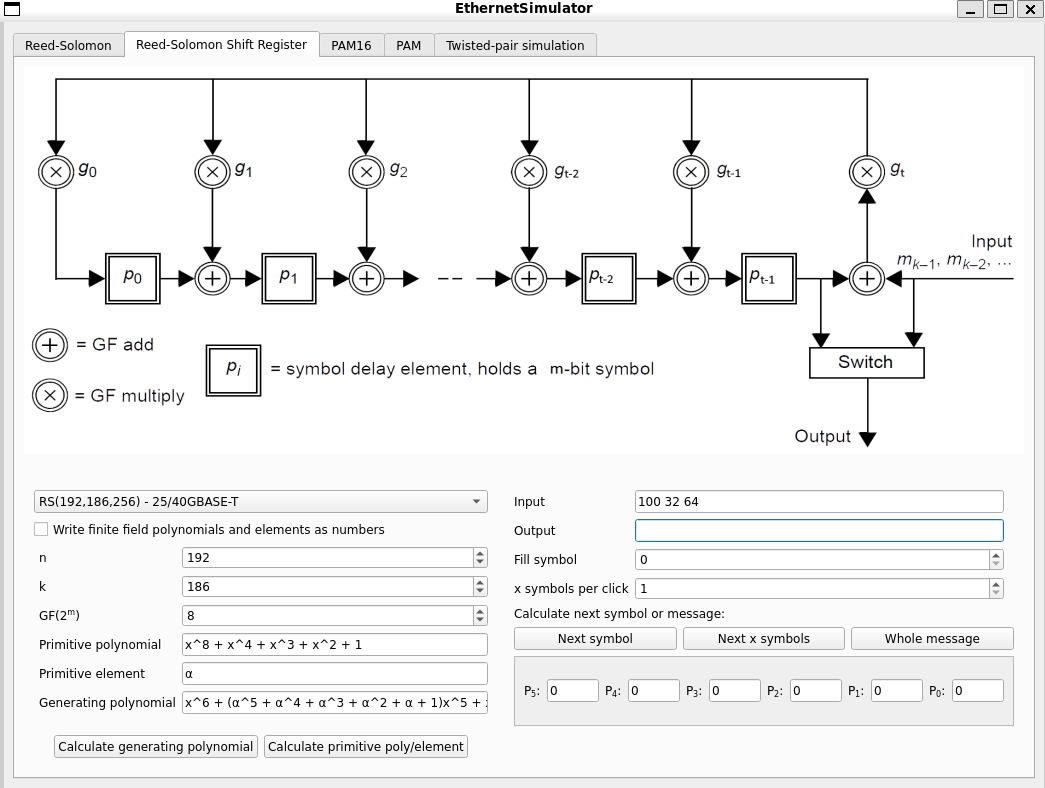
\includegraphics[width=0.95\textwidth,keepaspectratio]{rs-register-tab.png}
\end{center}
Narzędzie pozwala na:
\begin{itemize}
    \item Obliczanie wielomianu generującego kod Reeda-Solomona
    \item Zobrazowanie jak działa przykładowy koder Reeda-Solomona
    \item Zaznajomienie się z reprezentacją w postaci wielomianowej symboli z ciała $\mathbb{F}_{2^m}$
\end{itemize}

W tej zakładce koder RS zaimplementowany został zgodnie z modelem
funkcyjnym udostępnionym w standarcie Ethernet. Po przejściu
wszystkich symboli wiadomości element `Switch' zacznie przepuszczać symbole parzystości.
W opcjach po lewej możemy podobnie jak w poprzedniej zakładce wybrać
parametry kodera oraz dodatkowo wybrać inne wielomiany i elementy prymitywne. Przycisk `Calculate generating polynomial' obliczy
wielomian generujący a `Calculate primitive poly/ement' obliczy element i wielomian prymitywny dla podanego ciała skończonego $\mathbb{F}_{2^m}$.
Po prawej stronie mamy dane wejściowe oraz aktualny stan rejestrów $p_i$. `Fill symbol' jest symbolem który będzie wysyłany jeżeli zabraknie symboli na wejściu.

\subsubsection{Zadania}

\begin{itemize}
    \item Zakładka: Reed-Solomon, ustawienia programu: kod systematyczny BCH, $n=15$, $GF=2^4$.
    Dla $k \in \{ 2, 6, 10, 13 \}$ sprawdź wartość słowa kodowego dla k-symbolowej wiadomości zawierającej same zera. Dlaczego otrzymałeś takie słowa kodowe?
    \item Zakładka: Reed-Solomon, ustawienia programu: $n = 7$, $k = 3$, $GF = 2^3$,
    kod systematyczny BCH, tryb dziesiętny, wiadomość wejściowa `1 2 3'.
    Sprawdź dla błędów `3', `3 2', `3 2 1' oraz `3 2 1 4' czy dekoder jest w stanie
    wykryć błędy oraz czy jest w stanie je poprawić a jeżeli tak to czy poprawnie.
    Czy wiesz dlaczego pojawiły się rozbieżności między błędami poprawionymi a wykrytymi?
    \item Zakładka: Reed-Solomon Shift Register, ustawienia programu:
    $n = 3$, $k = 2$, $GF = 2^2$. Oblicz wielomiany prymitywne naciskając przycisk
    `Calculate primitive poly/element'.
    Zakoduj wiadomość: `2 1' w symulatorze po czym zakoduj wiadomość
    używając wzoru z sekcji `Systematyczny kod BCH'. Porównaj wyniki.
    \item Zakładka: Reed-Solomon, ustawienia programu: $n = 15$, $k=7$, $GF = 2^4$,
    kod systematyczny BCH.
    Zakoduj dowolną niezerową $k$-symbolową wiadomość. Sprawdź czy przesunięcia słowa kodowego
    (z użyciem strzałek przy słowie `encoded') także będą słowem kodowym.
\end{itemize}
